\begin{frame}[fragile]{Lengthening the Reach of Molecular Dynamics Simulations}
%\vspace{5mm}
%\hspace{-5mm}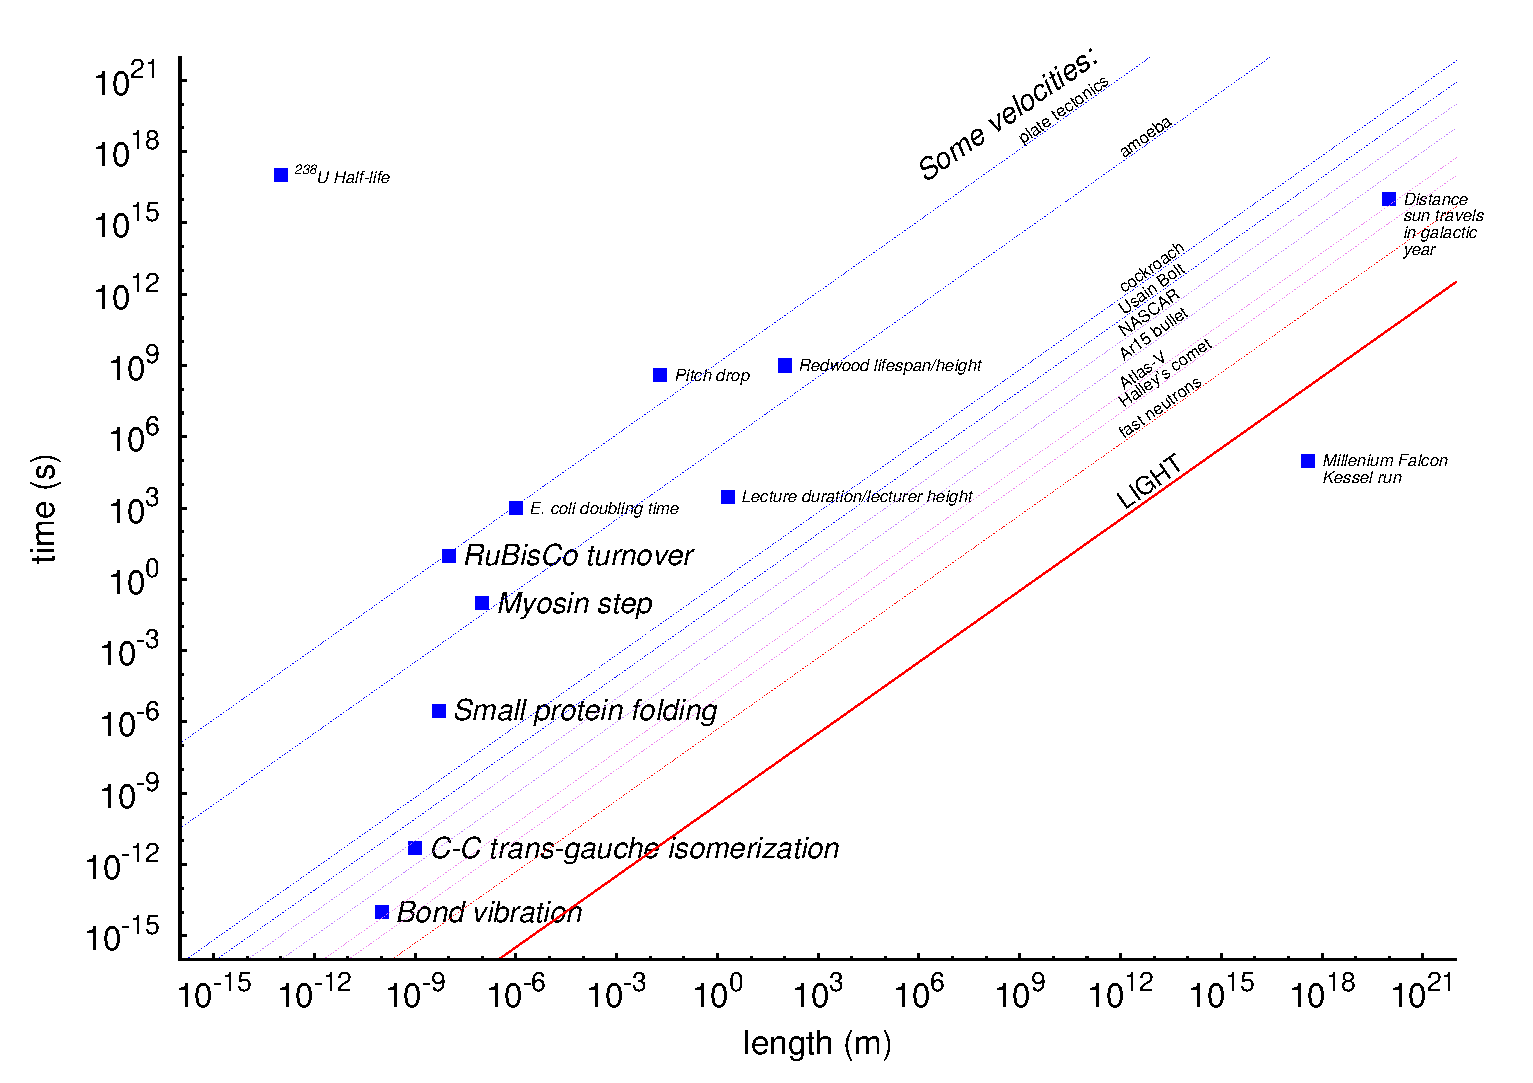
\includegraphics[width=\textwidth]{time_vs_length.eps}
\begin{tikzpicture}[scale=1.5]
\node[anchor=south west,inner sep=0] (image) at (0,0) 
{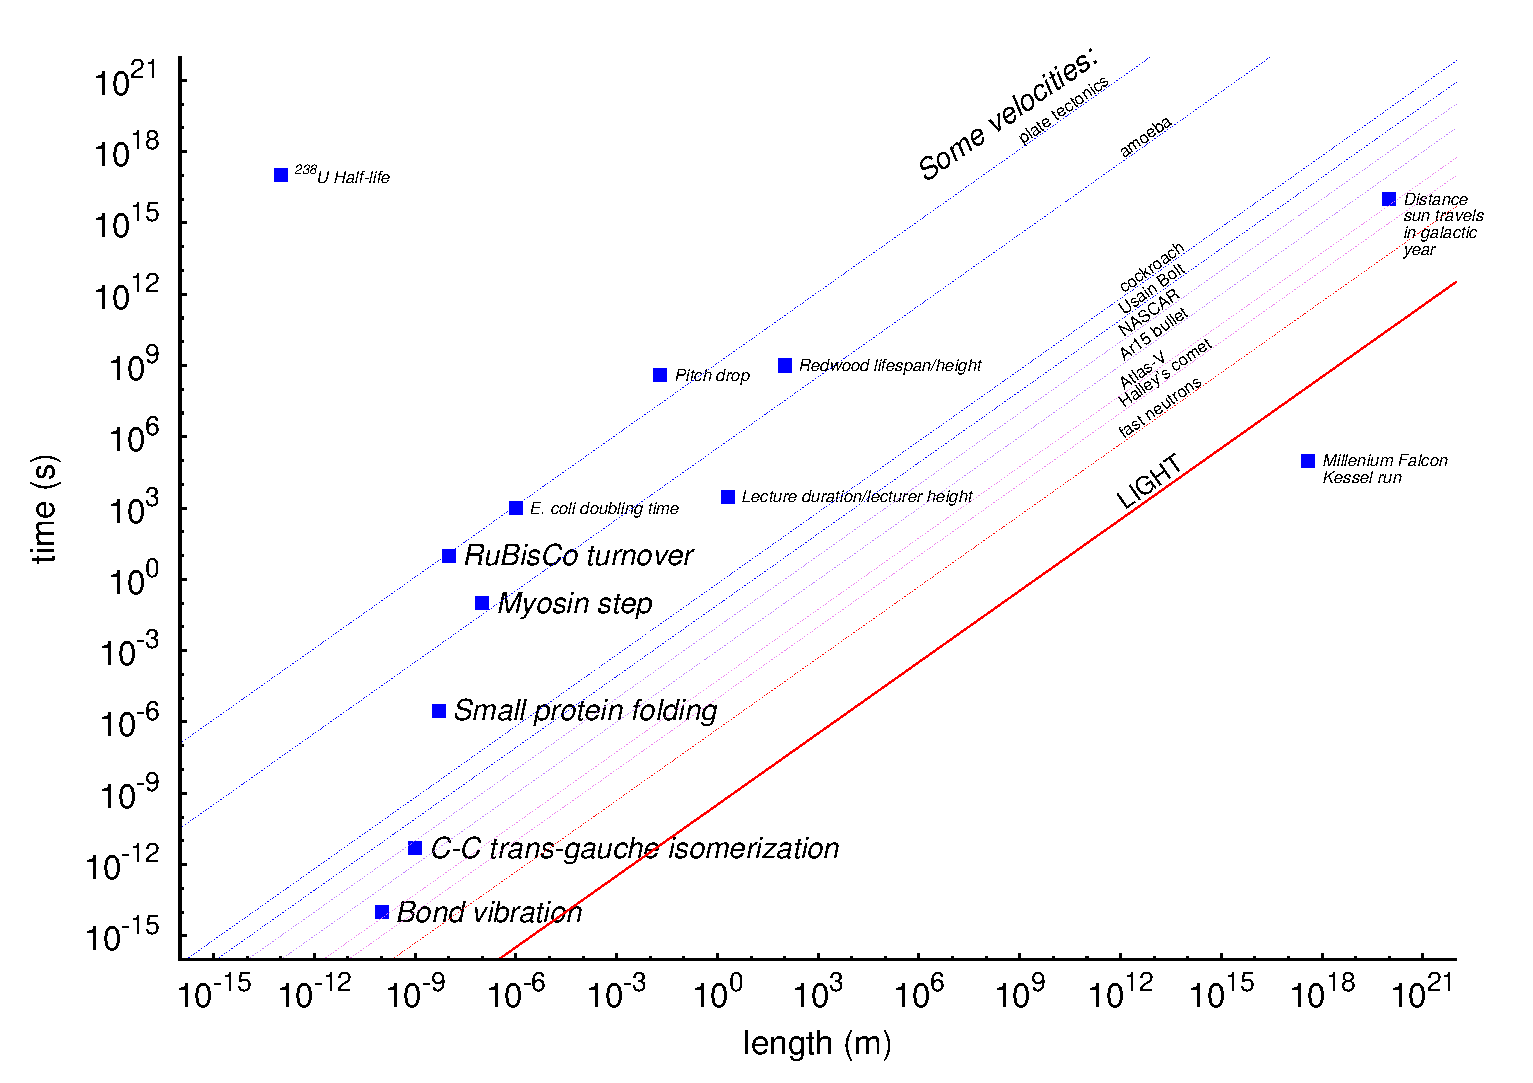
\includegraphics[width=0.975\textwidth]{time_vs_length.eps}};
\begin{scope}[x={(image.south east)},y={(image.north west)}]
\draw[red,thick,rounded corners] (0.2,0.125) rectangle (0.32,0.375);
\draw[red,thick] (0.26,0.275) node {MD};
\draw[->, green!80!black, thick, snake=snake, segment amplitude=.4mm, segment length=2mm, 
line after snake=1mm] (0.29,0.375) -- (0.29,0.45);
\draw[->, green!80!black, thick, snake=snake, segment amplitude=.4mm, segment length=2mm, 
line after snake=1mm] (0.26,0.375) -- (0.26,0.475);
\draw[->, green!80!black, thick, snake=snake, segment amplitude=.4mm, segment length=2mm, 
line after snake=1mm] (0.23,0.375) -- (0.23,0.5);
\draw[->, blue!80!white, thick, snake=snake, segment amplitude=.4mm, segment length=2mm, 
line after snake=1mm] (0.32,0.285) -- (0.38,0.285);
\draw[->, blue!80!white, thick, snake=snake, segment amplitude=.4mm, segment length=2mm, 
line after snake=1mm] (0.32,0.25) -- (0.4,0.25);
\node[green!80!black,text width=2cm,rotate=90] at (0.25,0.65) {Enhanced sampling};
%\draw [red,thick,rotate=-90] (0.3,0.6) node {Enhanced Sampling};
\draw [blue!80!white,thick] (0.57,0.27) node {Resolution coarsening};
\end{scope}
\end{tikzpicture}
\end{frame}

